\subsection{Modalities}

\begin{figure}
    \centering
    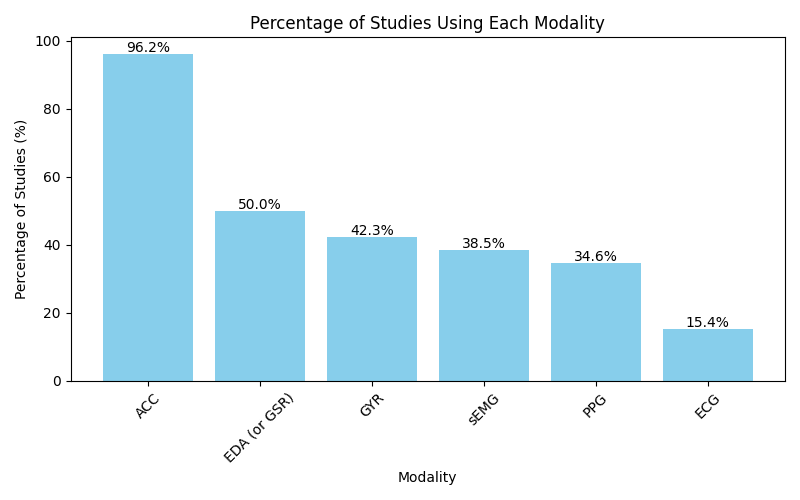
\includegraphics[width=1\textwidth]{Results/figures/percentage_of_studies_using_each_modality.png}
    \caption{Percentage of Studies Using Each Modality. Please note that studies used multiple sensors, however, the combination is not shown in this graph}
    \label{fig:percentage_of_studies_using_each_modality}
\end{figure}

\begin{figure}
    \centering
    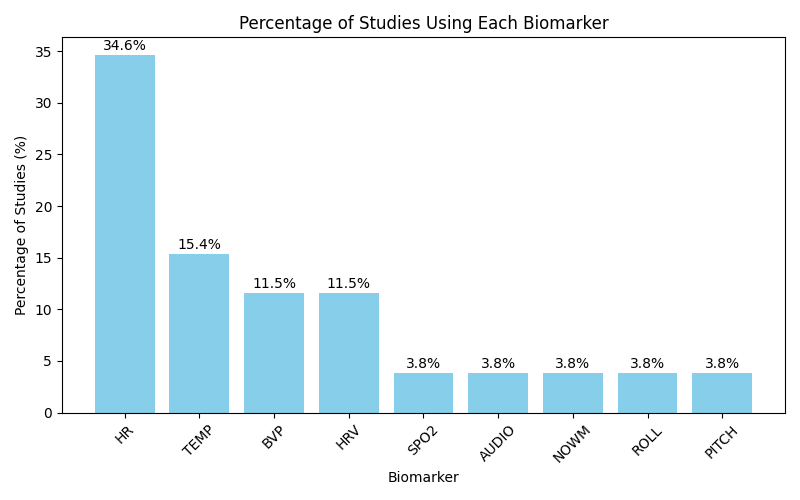
\includegraphics[width=1\textwidth]{Results/figures/percentage_of_studies_using_each_biomarker.png}
    \caption{Percentage of Studies Using Each Biomarker}
    \label{fig:percentage_of_studies_using_each_biomarker}
\end{figure}

\begin{figure}
    \centering
    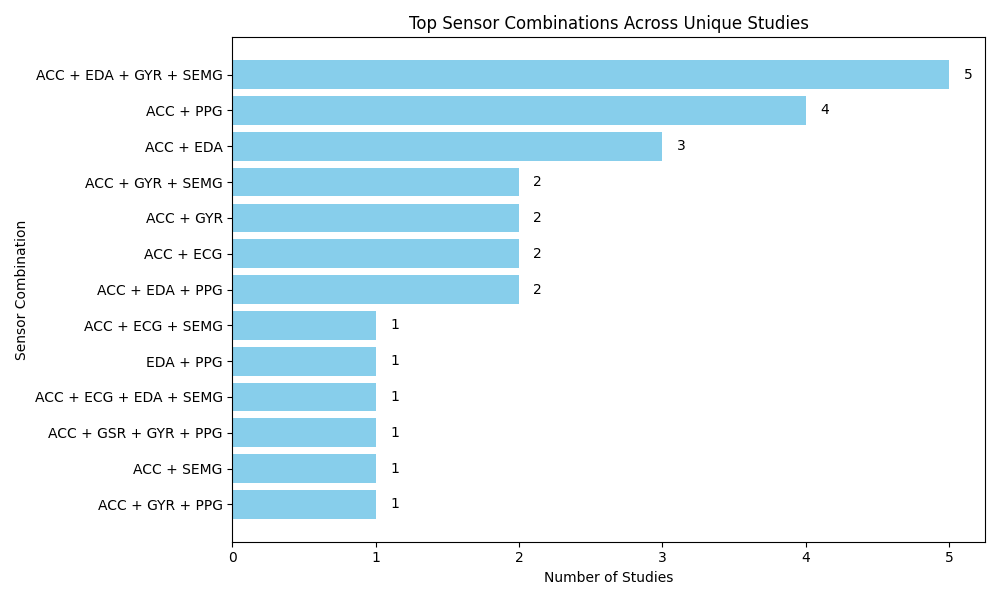
\includegraphics[width=1\textwidth]{Results/figures/freq_of_each_sensor_comp.png}
    \caption{Frequency of Each Sensor Combination}
    \label{fig:freq_of_each_sensor_comp}
\end{figure}

\subsubsection{Detection}
Among the 26 reviewed detection studies, ACC was by far the most frequently used modality (96.2\%) to capture the convulsive motor activity associated with tonic-clonic seizures. EDA followed as the second most used modality, appearing in half of the studies, while ECG was the least commonly used (15.4\%) (Figure \ref{fig:percentage_of_studies_using_each_modality}).

Several studies went beyond raw sensor signals and extracted specific biomarkers such as HR, HRV, BVP, and SpO$_2$, which were then used as features in seizure detection models. HR was the most commonly used biomarker (34.6\%), while SpO$_2$, audio, NOWM, and pitch and roll motion were each used in only 3.8\% of the studies (Figure \ref{fig:percentage_of_studies_using_each_biomarker}).

Altogether, 13 different multimodal sensor combinations were reported. The most common was ACC + GYR + sEMG + EDA (19.2\%; Figure \ref{fig:freq_of_each_sensor_comp}). Almost all studies that directly compared unimodal and multimodal systems \cite{Yu2023-ss,Milosevic2016-ee,De_Cooman2018-pq,Chowdhury2022-bi,Ge2023-ab, Wang2025-my,Tang2021-td,Li2022-ty,Hegarty-Craver2021-hk,Poh2012-af,Hamlin2021-sd,Wu2024-yl} found that multimodal systems outperformed unimodal ones. The only exception was \cite{Hegarty-Craver2021-hk}, where a cardiac algorithm using ECG alone achieved a lower FPR (1 per day) compared to ACC + ECG (2 per day).

The most commonly used multimodal sensor combination, ACC + GYR + sEMG + EDA \cite{Wang2025-ql, Ge2023-ab, Li2022-ty, Wu2024-yl, Wang2022-lt} consistently achieved high performance, with the highest reported in \cite{Wu2024-yl}. Among these studies, Wang et al. \cite{Wang2025-ql} investigated the use of derived biomarkers (PITCH and ROLL, extracted from ACC and GYR) instead of or in combination with raw ACC and GYR data. They found that substituting ACC with PITCH or ROLL improved performance across all models, with the best results obtained using SVM (Accuracy: 95.7\%, Precision: 95.7\%, Recall: 93.8\%; for ROLL: Accuracy: 95.2\%, Precision: 95.7\%, Recall: 92.5\%) compared to the original combination which achieved an accuracy of 93.4\%, precision of 95.8\%, and recall of 90.9\%. 

Another widely used combination was ACC + PPG \cite{Ali2020-ke, Tang2021-td, Arends2018-ew, Yu2023-ss}. Yu et al. \cite{Yu2023-ss} reported that for generalized motor seizures, ACC + BVP achieved the best performance with a mean AUC-ROC of 0.805, while EDA had the lowest mean AUC-ROC of 0.513. For tonic–clonic seizures, ACC alone achieved the best performance, with an AUC-ROC of 0.973, a sensitivity of 95\%, and FPR of 6.2\%. Similarly, Tang et al. \cite{Tang2021-td} reported that when ACC data was used alone, this model performed best for tonic-clonic seizures with an AUC-ROC of 0.995, however, for seizure type agnostic, ACC + BVP fusion performed best, with an AUC-ROC of 0.752. Another study \cite{Arends2018-ew}, an in-home nocturnal cohort study, reported that their sensitivity was significantly high (median 85\%) compared to a rhythmic movement-based bed sensor (median 21\%). They further analyzed feature contributions and showed that HR was the critical modality for true positives (92\%) and also for false positives, while ACC contributed only 8\% of true positives and caused no false alarms.

ACC + EDA was also one of the top and high achieving combinations \cite{Regalia2019-ch, Poh2012-af, Chowdhury2022-bi} with the highest sensitivity (97.2\%) reported by \cite{Chowdhury2022-bi} and the lowest FAR/24h (0.53) reported by \cite{Regalia2019-ch}, which validated Empatica multimodal wristbands (E4 and Embrace) as reliable tools for GTCS detection in real-world and Epilepsy Monitoring Units (EMUs) settings. Chowdhury et al. \cite{Chowdhury2022-bi} reported that fusing ACC and EDA significantly improved classification accuracy (96.7\%) and reduced FAR (unspecified) compared to unimodal approaches. Similarly, Poh et al. \cite{Poh2012-af} reported that the overall performance was lower when only ACC features were included.

While most studies incorporate both physiological and motion-based sensors in their sensor suite, 19.2\% of the studies were purely motion-based, using sensor combinations of ACC + GYR \cite{Larsen2024-vn, Dong2022-oo}, ACC + GYR + sEMG \cite{Wang2025-my, Gheryani2017-yg} and ACC + sEMG \cite{Milosevic2016-ee}. Among these, the ACC + sEMG + GYR configuration achieved the best performance. In addition to studying their significance in seizure detection, a few studies have tested for the optimal sensor placement \cite{Milosevic2016-ee, De_Cooman2018-pq}, showing that using sensors on different body locations can reduce false alarms and improve performance. \cite{Milosevic2016-ee} identified the left wrist (generally the non-dominant hand) and right ankle as optimal positions for ACC sensors, while bilateral biceps were optimal for sEMG. 

For details of the remaining reported combinations, refer to the Modality Table.

\subsubsection{Prediction and Forecasting}
All three studies used EDA and PPG in their sensor suite. One seizure forecasting study additionally used ACC \cite{Meisel2020-ii}. PPG was used to extract biomarkers like HR in \cite{Vieluf2023-ta, Vieluf2023-zv}, HRV in \cite{Vieluf2023-zv}, and BVP in \cite{Meisel2020-ii}. TEMP was also among the biomarkers used by \cite{Vieluf2023-zv, Meisel2020-ii}, however in \cite{Vieluf2023-zv}, TEMP did not differ between seizure and non-seizure groups and was therefore not included in further analysis. Vieluf et al. \cite{Vieluf2023-ta, Vieluf2023-zv} identified EDA and HR as containing sufficient seizure-predictive information, with reported performance of 62\% sensitivity and an accuracy range of 68–68.89\%. These findings were further supported in \cite{Vieluf2023-zv}, where HRV was additionally shown to carry predictive value: patients with an impending seizure had lower HR and higher HRV compared to seizure-free patients in evening recordings. In \cite{Meisel2020-ii}, forecasting performance was highest when all modalities (EDA, BVP, TEMP, ACC) were combined achieving significant seizure forecasting (better-than-chance) in 43\% of patients (30/69), where the mean sensitivity was 75.6\%, the mean time in warning (TiW) was 47.2\% and the mean prediction horizon was 31.6 minutes. Each modality contributed uniquely, though accelerometry sometimes reduced performance in low-performing patients